\documentclass{article}
\usepackage{graphicx} % Required for inserting images
\usepackage{amsmath}
\usepackage{amssymb}
\usepackage[section]{placeins}
\usepackage{subfigure}
\usepackage{biblatex}
\addbibresource{biblio.bib}
\usepackage{multicol}
\setlength{\columnsep}{1cm}
\usepackage[bottom=1.5cm, right=1.5cm, left=1.5cm, top=3cm]{geometry}

\title{Notes de stage \\}
\date{}

\begin{document}

\maketitle

\begin{abstract}
    Simulation et estimation de la diffraction d'un élément en condition de faible
    intensité par des méthodes probabilistiques de compte de photons
\end{abstract}


\section{Modèle}

Le résultat en sortie de simulation est un array de 3 dimensions, composé de $M$ tableaux de taille $N*N$, où $M$ correspond au nombre de frames enregistrées et N le nombre de pixels sur un côté du détecteur. \\
On modèlise l'intensité sur le détecteur $X$ par une loi Gamma $G$ de nombre de modes $L_X$ et de moyenne $i$, où $i$ est le tirage de l'intesité du faisceau pour cette frame : $X \thicksim G(L_X, i)$ \\
Pour compter les photons qui ont impacté le détecteur $Y$ nous utilisons une loi de Poisson $P$ sur un tirage de l'intensite : $Y \thicksim P(X)$ \\

Les différences entre les modèles se font sur la modélisation du faisceau et en second temps la modélisation de la diffraction.

\subsection{Base: Intensité constante}

On estime que le faiceau est d'intensité constante $\bar{I}$. \\
L'intensité sur détecteur suit une loi Gamma $G(L_X, \bar{I})$
En composant avec la loi de Poisson ,on obtient un compte de photon suivant une loi négative binomiale\cite[p.~81]{teich_multiply_1989} : $Y \thicksim NB(L_X, \bar{I})$ \\

Leurs fonctions de masse respectivent sont\cite[p.~83-84]{teich_multiply_1989} :

\begin{align}
    &g(x, L_X, \bar{I}) = \frac{1}{\Gamma(L_X)} \bigg( \frac{L_X}{\bar{I}} \bigg) ^{L_X} x^{L_X-1} \exp{\frac{-L_Xx}{\bar{I}}} \\
    &b(y, L_X, \bar{I}) = \frac{(L_X)^{L_X}}{\Gamma(L_X)} \frac{\Gamma(y+L_X)}{y!} \frac{\bar{I}^y}{(\bar{I} L_X)^{y+L_X}}
\end{align}

Graphes produits avec $N = 128; M = 1500$.
Les images sont celles du premier tirage des lois et les histogrammes comprennent l’ensemble des frames.

\begin{figure}
    \centering

    \subfigure[]{
    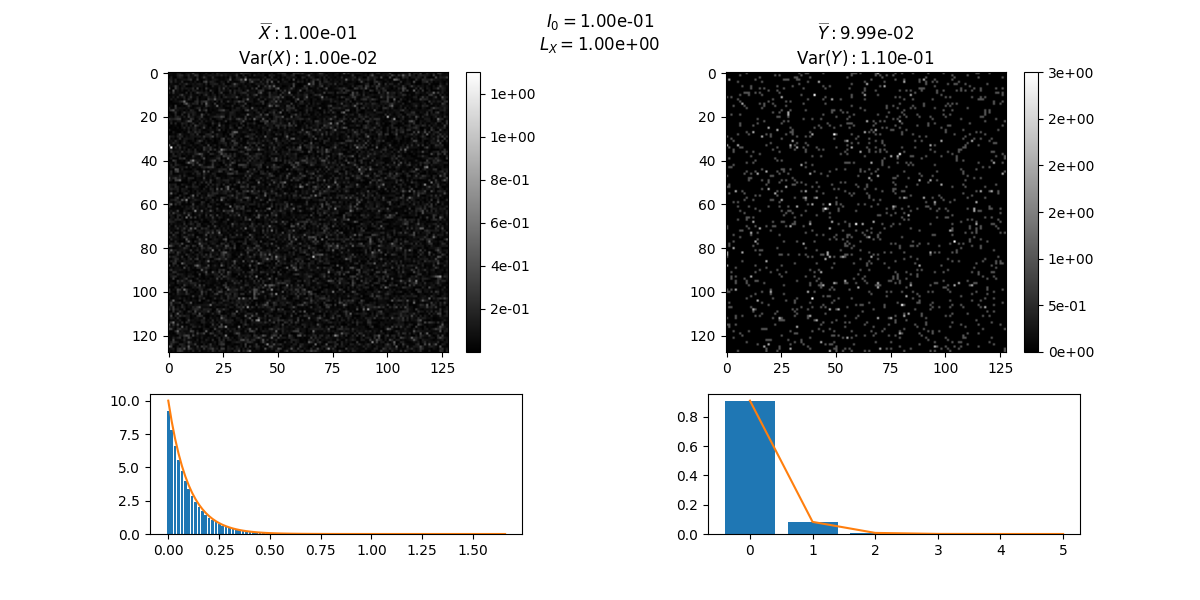
\includegraphics[width=0.45\linewidth]{graphs/modele_base/I0_0,1_Lx_1.png}}
    \subfigure[]{
    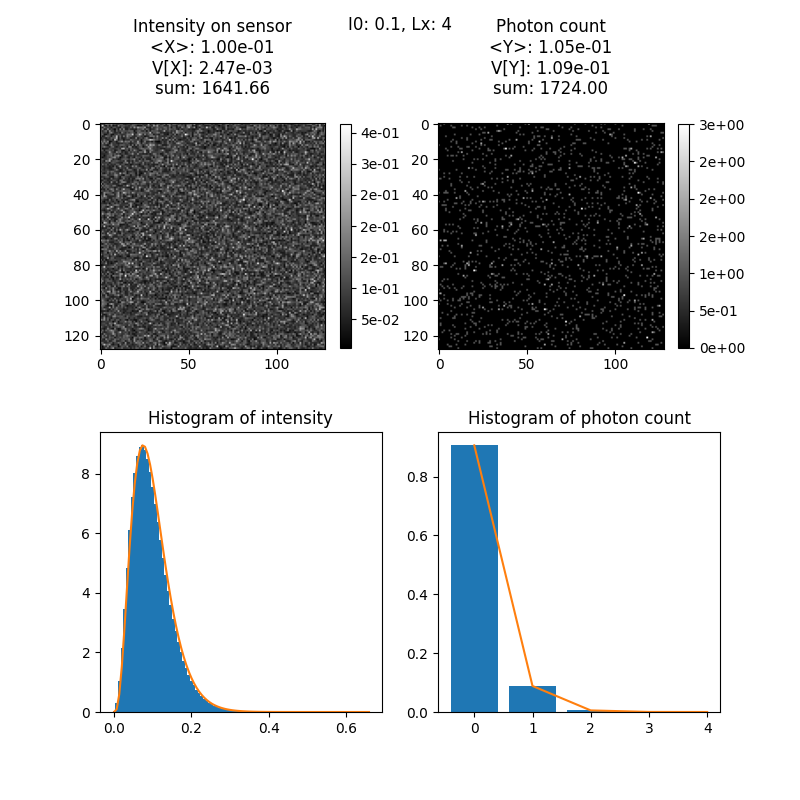
\includegraphics[width=0.45\linewidth]{graphs/modele_base/I0_0,1_Lx_4.png}}
    
    \caption{Simulations avec $I_0 = 0.1$}
\end{figure}

\begin{figure}
    \centering
    
    \subfigure[]{
    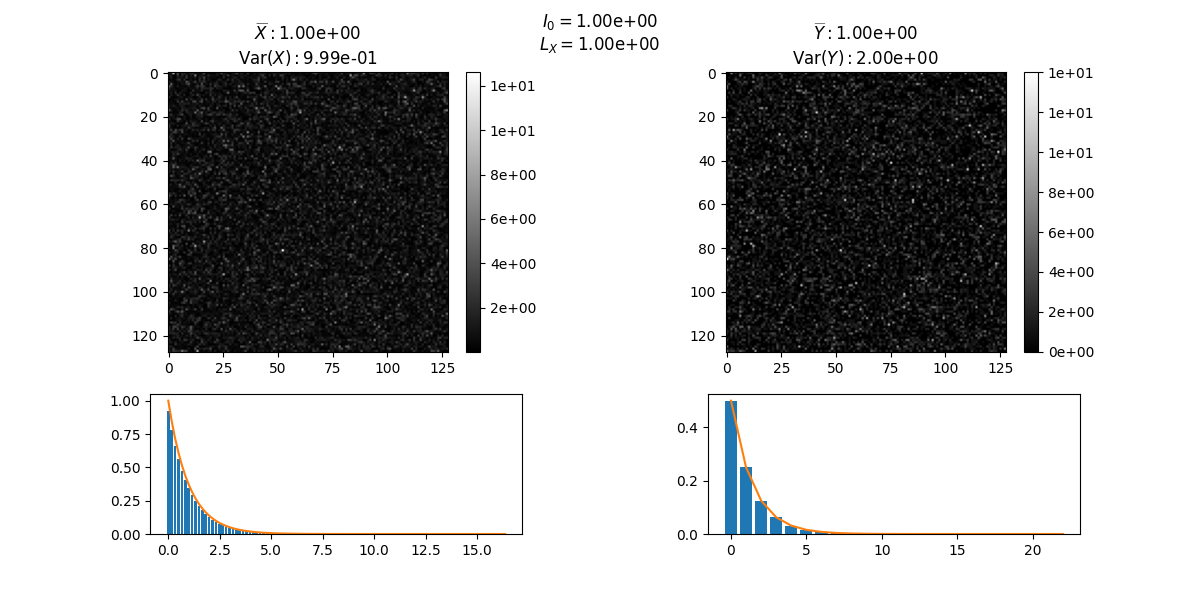
\includegraphics[width=0.45\linewidth]{graphs/modele_base/I0_1_Lx_1.png}}
    \subfigure[]{
    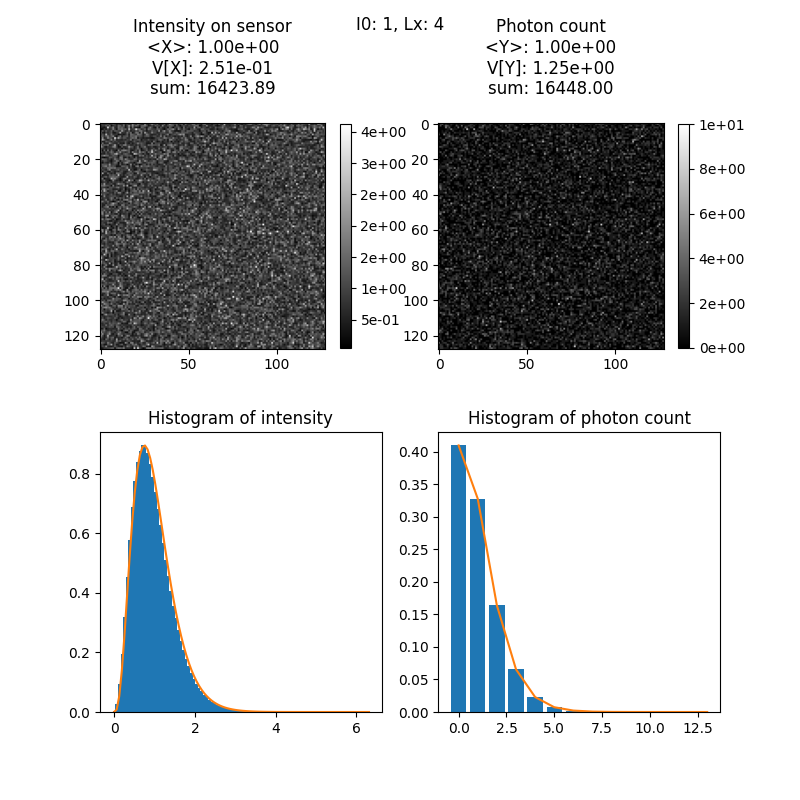
\includegraphics[width=0.45\linewidth]{graphs/modele_base/I0_1_Lx_4.png}}
    
    \caption{Simulations avec $I_0 = 1$}
\end{figure}

\begin{figure}
    \centering

    \subfigure[]{
    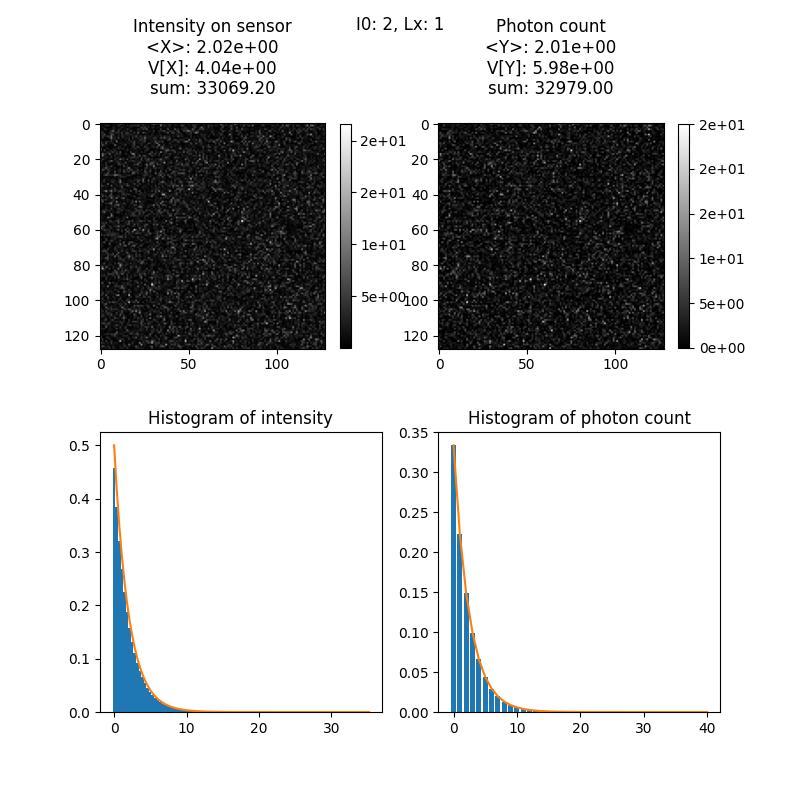
\includegraphics[width=0.45\linewidth]{graphs/modele_base/I0_2_Lx_1.png}}
    \subfigure[]{
    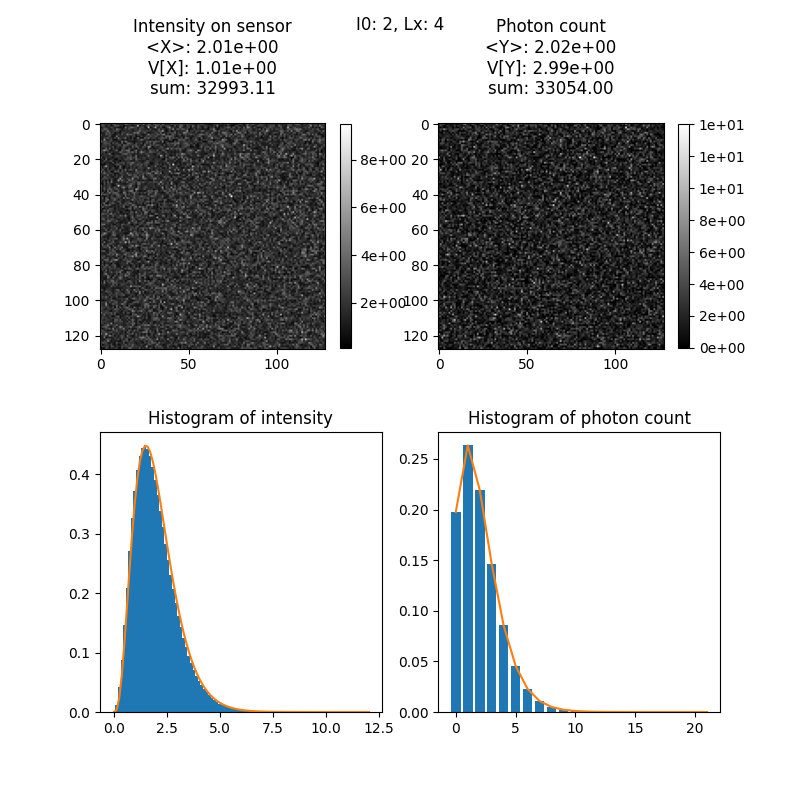
\includegraphics[width=0.45\linewidth]{graphs/modele_base/I0_2_Lx_4.png}}
    
    \caption{Simulations avec $I_0 = 2$}
\end{figure}

\FloatBarrier

\subsubsection{Estimation}

Les moments fractionnels de la loi Gamma-Poisson sont égaux aux moments de la loi Gamma\cite[p.~83]{teich_multiply_1989} :
$$
<f(y, m)> = <x^m> = \bar{I}^m \frac{\Gamma(L_X + m)}{L_X^m \Gamma(L_X)}
$$

On peut donc calculer les deux premiers moments théoriques:
$$
< x > = \bar{I} ; \quad < x^2 > = \frac{\bar{I}}{L_X}
$$

Et estimer les paramètres $\bar{I}$ et $L_X$ à partir des deux premiers moments empyriques :
$$
\bar{I}’ = < x > = < y > ; \quad L_X' = \frac{<x>^2}{<x^2> - <x>^2} = \frac{<y>^2}{<y(y-1)> - <y>^2}
$$

\subsection{Fluctuaction de l'intensité}

On modèlise le faisceau par une loi Gamma : $I \thicksim G(L_I, \bar{I})$, avec $L_I$ le nombre de modes 




\section{Codes}

L’ensemble du code est disponible sur GitHub à l’adresse : https://github.com/louise-aresu/spectrEchantillon

\printbibliography

\end{document}
